\clearpage
\section*{Appendix. Reproduction and complete source listings}
\phantomsection
\addcontentsline{toc}{section}{Appendix. Reproduction and complete source listings}
Python 3.12.14, CatBoost 1.2.10, pymatgen 2025.10.7, NumPy 2.5.5, pandas 2.2.3, SciPy 1.18.1, scikit-learn 1.9.1 and Kaiwu SDK 1.4.4 were used on Windows 11. Figures use the ideal cubic prototype, public physical properties, saved predictions and solver tables. The revised figures were rendered from the archived values with Matplotlib 3.10.8 and typeset with XeLaTeX and the APMCM class.

Place the original files in \texttt{problem\_d/date}. Run the data audit, the validation and stress comparisons for seeds 26 and 42, the physical-property comparison, the seed-26 encoding and precision audit, then the paper scripts. Running \texttt{screen.py scores} produces the hidden Q1 predictions and the refit Q2/Q3 score table. Running \texttt{screen.py development} produces the five-fold results. Use \texttt{solve.py} for both full-pool searches, \texttt{gate\_audit.py} for the gate replay, \texttt{capacity\_audit.py} for the direct-model controls and \texttt{mechanisms.py} for the consistency and margin checks. Run \texttt{figures.py}, \texttt{material\_figures.py}, \texttt{perovskite\_plates.py}, \texttt{crystal\_scenes.py} and \texttt{tables.py} for the manuscript. The companion README gives the arguments and file names for each call.

The score ledger records SHA-256 digests for the two exported tables. The block ledger contains the selected ID, tie count, integer-energy minimum, scaled Ising energy, observed coupling range and timing for each call. Both final-pool selections can be reconstructed from the tables alone.

\setcounter{figure}{0}
\renewcommand{\thefigure}{A\arabic{figure}}
\renewcommand{\theHfigure}{supp.\arabic{figure}}
\subhead{Screening curves by candidate pool}
\begin{figure}[htbp]
\centering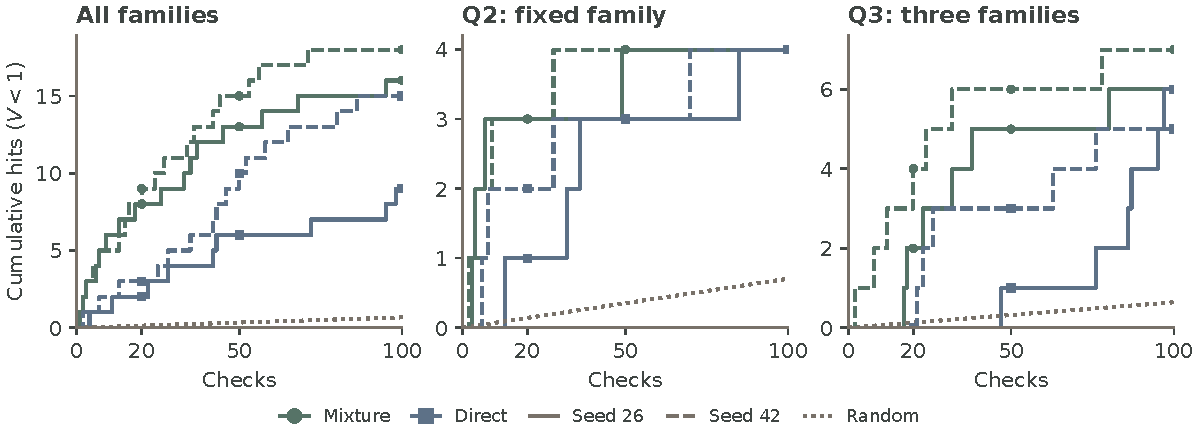
\includegraphics[width=\linewidth]{figures/screening.pdf}
\caption{Cumulative $V<1$ hits on file 03. Circles indicate the mixture, squares direct regression, solid lines seed 26 and dashed lines seed 42. The dotted line gives the expected cumulative count under random selection.}\label{fig:allbudgets}
\end{figure}
\subhead{Family choices for the blind candidate}
For the blind finalist, fixing La on A and Ti on B leaves three distinct compositions in the Q3 pool. Their anion fractions, in the order O, N, F, are $(1,0,0)$, $(2/3,1/3,0)$ and $(2/3,0,1/3)$. Equation~\eqref{eq:envelope} takes the minimum over these three discrete alternatives. Figure~\ref{fig:families} compares their stoichiometry and frozen scores. The data give no site-resolved geometry for the blind material.

\begin{figure}[htbp]
\centering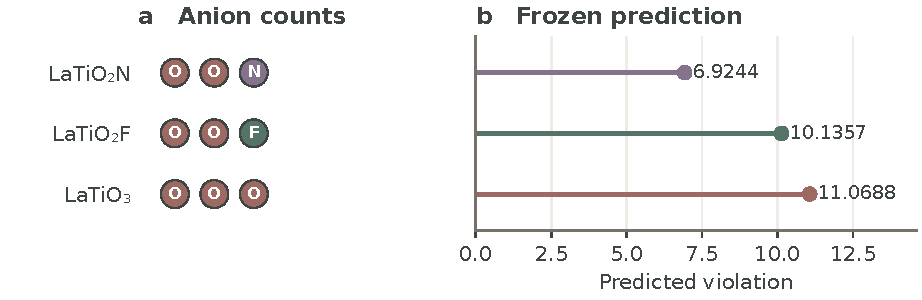
\includegraphics[width=\linewidth]{figures/anion_substitution.pdf}
\caption{Three anion compositions for the same La--Ti pair. Symbols count anions per formula unit. Predictions come from the refitted Q3 score table. The physical violation of the blind recommendation remains unknown.}\label{fig:families}
\end{figure}

The three minima share Ti on the B site and differ at A. They are $(\mathrm{Sn},\mathrm{Ti})$ at 3.268113 in O3, $(\mathrm{La},\mathrm{Ti})$ at 6.924382 in NO2, and $(\mathrm{Ca},\mathrm{Ti})$ at 4.585642 in FO2. Eight of the ten lowest scores across the full three-family pool also place Ti at B. This concentration describes the frozen surrogate. The ten records are selected extremes and cannot establish a general causal effect of Ti.

Holding La and Ti fixed, switching from NO2 to FO2 increases the score from 6.9244 to 10.1357, and switching to O3 raises it to 11.0688. Across all 2,704 pairs, however, O3 supplies the smallest score in 2,188 cells, NO2 in 378 and FO2 in 138. Each cell has a unique family minimum in the stored table. Thus choosing the family with the most pairwise wins would overlook the preferred family for the blind finalist.

The public Q3 winner also allows a physical check. Its formation energy of 0.10 eV, gap of 2.50 eV and VBM of 6.998833 eV all pass the corresponding thresholds. Its CBM of 4.518833 eV exceeds 4.50 by only 0.018833 eV, accounting for its entire reported violation. For the blind $\mathrm{LaTiO_2N}$ candidate, only composition and surrogate rank are observed. A new physical calculation would be needed to identify its limiting property.

\FloatBarrier
\lstset{language=Python,basicstyle=\fontsize{8.5}{10}\selectfont\ttfamily,
  columns=fullflexible,keepspaces=true,breaklines=true,breakatwhitespace=false,
  frame=none,backgroundcolor=\color{white},rulecolor=\color{white},
  keywordstyle=\color{black},stringstyle=\color{black},commentstyle=\color{black!65},
  aboveskip=2pt,belowskip=4pt,showstringspaces=false}
\newcommand{\program}[2]{\par\addvspace{1.2\baselineskip}\Needspace{8\baselineskip}\subhead{#1}\lstinputlisting{#2}}
\program{A1. Surrogate features and model components}{../exploration/compare_surrogates.py}
\program{A2. Source checks and label reconstruction}{../exploration/audit_data.py}
\program{A3. Withheld near-target and encoding experiments}{../exploration/test_innovation_ideas.py}
\program{A4. Physical-property-first prediction}{../exploration/compare_physical_properties.py}
\program{A5. Whole-grid SDK precision audit}{../exploration/audit_sdk_precision.py}
\program{A6. Frozen predictions and grouped folds}{screen.py}
\program{A7. Integer QUBO construction, exact solution and checks}{solve.py}
\program{A8. Manuscript figures}{figures.py}
\program{A9. Measured values for the manuscript tables}{tables.py}
\program{A10. Crystal geometry and screening diagnostics}{material_figures.py}
\program{A11. Perovskite structure, band edges and anion compositions}{perovskite_plates.py}
\program{A12. Gap-gate replay and validation ablation}{gate_audit.py}
\program{A13. Consistency and margin diagnostics}{mechanisms.py}
\program{A14. Weighted gate and QUBO readout}{crystal_scenes.py}
\program{A15. Direct-regression capacity controls}{capacity_audit.py}
